\documentclass[a4paper,12pt]{article}
\usepackage[T2A]{fontenc}
\usepackage[utf8x]{inputenc}
\usepackage[english,russian]{babel}
\usepackage{amssymb,amsfonts,amsmath,mathtext}
\usepackage[unicode]{hyperref}
\usepackage{listings}
\usepackage{graphicx}
\graphicspath{{images/}}
\newcommand{\anonsection}[1]{\section*{#1}\addcontentsline{toc}{section}{#1}}

\begin{document}

% Титульный лист

\begin{titlepage}
\newpage

\begin{center}

\textit{Министерство науки и высшего образования Российской Федерации \\ 
Федеральное государственное бюджетное образовательное \\
учреждение высшего образования \\
«Московский государственный технический университет \\
имени Н.Э. Баумана (национальный исследовательский университет)» \\
(МГТУ им. Н.Э. Баумана) \\}
\hrulefill
\end{center}

\vspace{2em}

\begin{flushleft}
ФАКУЛЬТЕТ <<Информатика и системы управления>> \\
\vspace{0.5em}
КАФЕДРА <<Программное обеспечение ЭВМ и информационные технологии>>
\end{flushleft}


\vspace{8em}

\begin{center}
\LARGE Лабораторная работа №2 \\
\end{center}

\vspace{1.5em}

\begin{center}
\textsc{Умножение матриц}
\end{center}

\vspace{6em}

\begin{center}
Головнев Н.В.

\vspace{4em}

ИУ7-54Б
\end{center}

\vspace{\fill}

\begin{center}
Москва 2019
\end{center}

\end{titlepage}

\tableofcontents

% Введение

\newpage
\anonsection{ВВЕДЕНИЕ}

\begin{flushleft}
Цель данной лабораторной работы:\\
% Вставь сюда цель лабораторной работы
Постановка задачи:\\
\begin{enumerate}
\item Реализовать классический алгоритм умножения матриц
\item Реализовать алгоритм умножения матриц методом Винограда
\end{enumerate}
\end{flushleft}

% Аналитическая часть

\newpage
\section{АНАЛИТИЧЕСКАЯ ЧАСТЬ}
\subsection{Описание алгоритмов}
% Поищи книжки

\newpage
\subsection{Вывод}
% Напиши для начала описание алгоритмов, а уже потом пиши эту каку

% Конструкторская часть

\newpage
\section{КОНСТРУКТОРСКАЯ ЧАСТЬ}

\subsection{Разработка алгоритмов}
% Что подается на вход, выход и тд

\newpage
\subsection{Схемы алгоритмов}
% Как же я ненавижу делать эти схемы

\newpage
\subsection{Вывод}
% Для начала надо сделать предыдущее

\newpage
\section{ТЕХНОЛОГИЧЕСКАЯ ЧАСТЬ}
\subsection{Требования к программному обеспечению}

\begin{flushleft}
Программа должна работать на операционной системе Arch Linux. Программа должна
содержать 2 режима:
\begin{itemize}
\item Пользовательский
\item Экспериментальный
\end{itemize}
В пользовательском режиме пользователь должен иметь возможность вводить матрицы и получать на выходе результаты работ всех реализованных алгоритмов умножения матриц. В экспериментальном режиме засекается процессорное время работы каждого алгоритма, результаты записываются в отдельные файлы. Впоследствии данные из этих файлов можно вывести в виде графика зависимости процессорного времени от размеров матриц.
\end{flushleft}

\newpage
\subsection{Средства реализации}
Для реализации данных алгоритмов был выбран язык программирования С, компилятор
gcc и некоторые функции из библиотеки glibc (memcpy, malloc и тд...). \\
Удобства, предоставляемые языком C:
\begin{itemize}
\item Прямой доступ к памяти;
\item Возможность составлять простейшие структуры данных;
\end{itemize}
Для вывода графиков использовался Python3 (библиотека Matplotlib)

\newpage
\subsection{Листинг кода}
Ниже приведены реализации алгоритмов на С.\\
\lstdefinestyle{customc}{
  belowcaptionskip=1\baselineskip,
  breaklines=true,
  frame=L,
  xleftmargin=\parindent,
  language=C,
  showstringspaces=false,
  basicstyle=\footnotesize\ttfamily
}

% В директории надо добавить листинги с кодом
%\lstinputlisting[captionpos=b, caption=\label{listings:listing1}Стандартная реализация алгоритма Левенштейна(\ref{images:levenstein}), style=customc]{listing1.c}
\newpage
%\lstinputlisting[captionpos=b, caption=\label{listings:listing2}Рекурсивная реализация алгоритма Левенштейна(\ref{images:recursive_levenstein}), style=customc]{listing2.c}
\newpage
%\lstinputlisting[captionpos=b, caption=\label{listings:listing3}Стандартная реализация алгоритма Дамерау-Левенштейна(\ref{images:damerau_levenstein}), style=customc]{listing3.c}

\newpage
\subsection{Вывод}
Используя язык программирования C, в ходе практической работы были спроектированы и написаны реализации алгоритмов умножения матриц. Используя эти реализации были написаны 2 приложения: пользовательское приложение и приложение для подсчета процессорного времени выполнения этих алгоритмов.

\newpage
\section{ЭКСПЕРИМЕНТАЛЬНАЯ ЧАСТЬ}
\subsection{Характеристики аппаратного и программного обеспечения}
\flushleft{Тестирование приложения проводилось на машине со следующими характеристиками:\\}
\begin{itemize}
\item Процессор Intel® Core™ i7-7700HQ;
\item Оперативная память 16 ГБ;
\item Операционная система - Arch Linux с рабочим окружением Gnome 3.
\end{itemize}

\newpage
\subsection{Примеры работы}
\begin{flushleft}
На Рис., предсавленном ниже, демонстрируется работа приложения. Запуск приложения осуществляется из эмулятора терминала в Arch Linux. Во время работы приложение запрашивает у пользователя ввод параметров матриц, а также ввод отдельных строк каждой матрицы. На выходе она печатает
\end{flushleft}
\begin{figure}[h]
\center{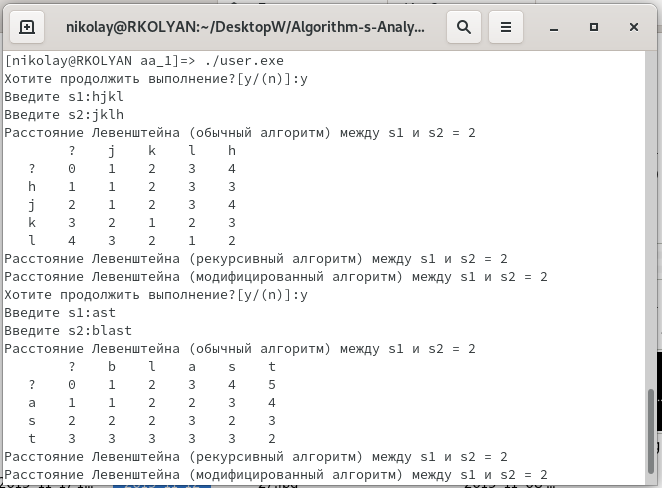
\includegraphics[scale=0.5]{example.png}}
\caption{Пример работы приложения}
\label{images:example}
\end{figure}

\newpage
\subsection{Результаты тестирования}
% Не знаю как, но нужно здесь показать небольшие результаты тестирования.

\newpage
\subsection{Постановка эксперимента по замеру времени}
\begin{flushleft}
Для вычисления процессорного времени работы алгоритмов использовалась функция clock(), объявленная в заголовочном файле time.h из библиотеки glibc. \\
Требования к программе, считающей время выполнения алгоритмов:
\begin{itemize}
\item Ввод пользователем таких параметров, как:
\begin{itemize}
\item Максимальная длина стороны обоих матриц;
\item Кол-во итераций на каждый рассматриваемый случай (для высчитывания среднего значения);
\end{itemize}
\item Матрицы генерируются со случайными числами;
\item Результаты вычислений должны сохранятся в текстовых файлах.
\end{itemize}
\end{flushleft}

\newpage
\subsection{Сравнительный анализ на материале экспериментальных данных}
% Картинку надо поменять и вставить к ней соответствующий текст

\begin{figure}[h]
\center{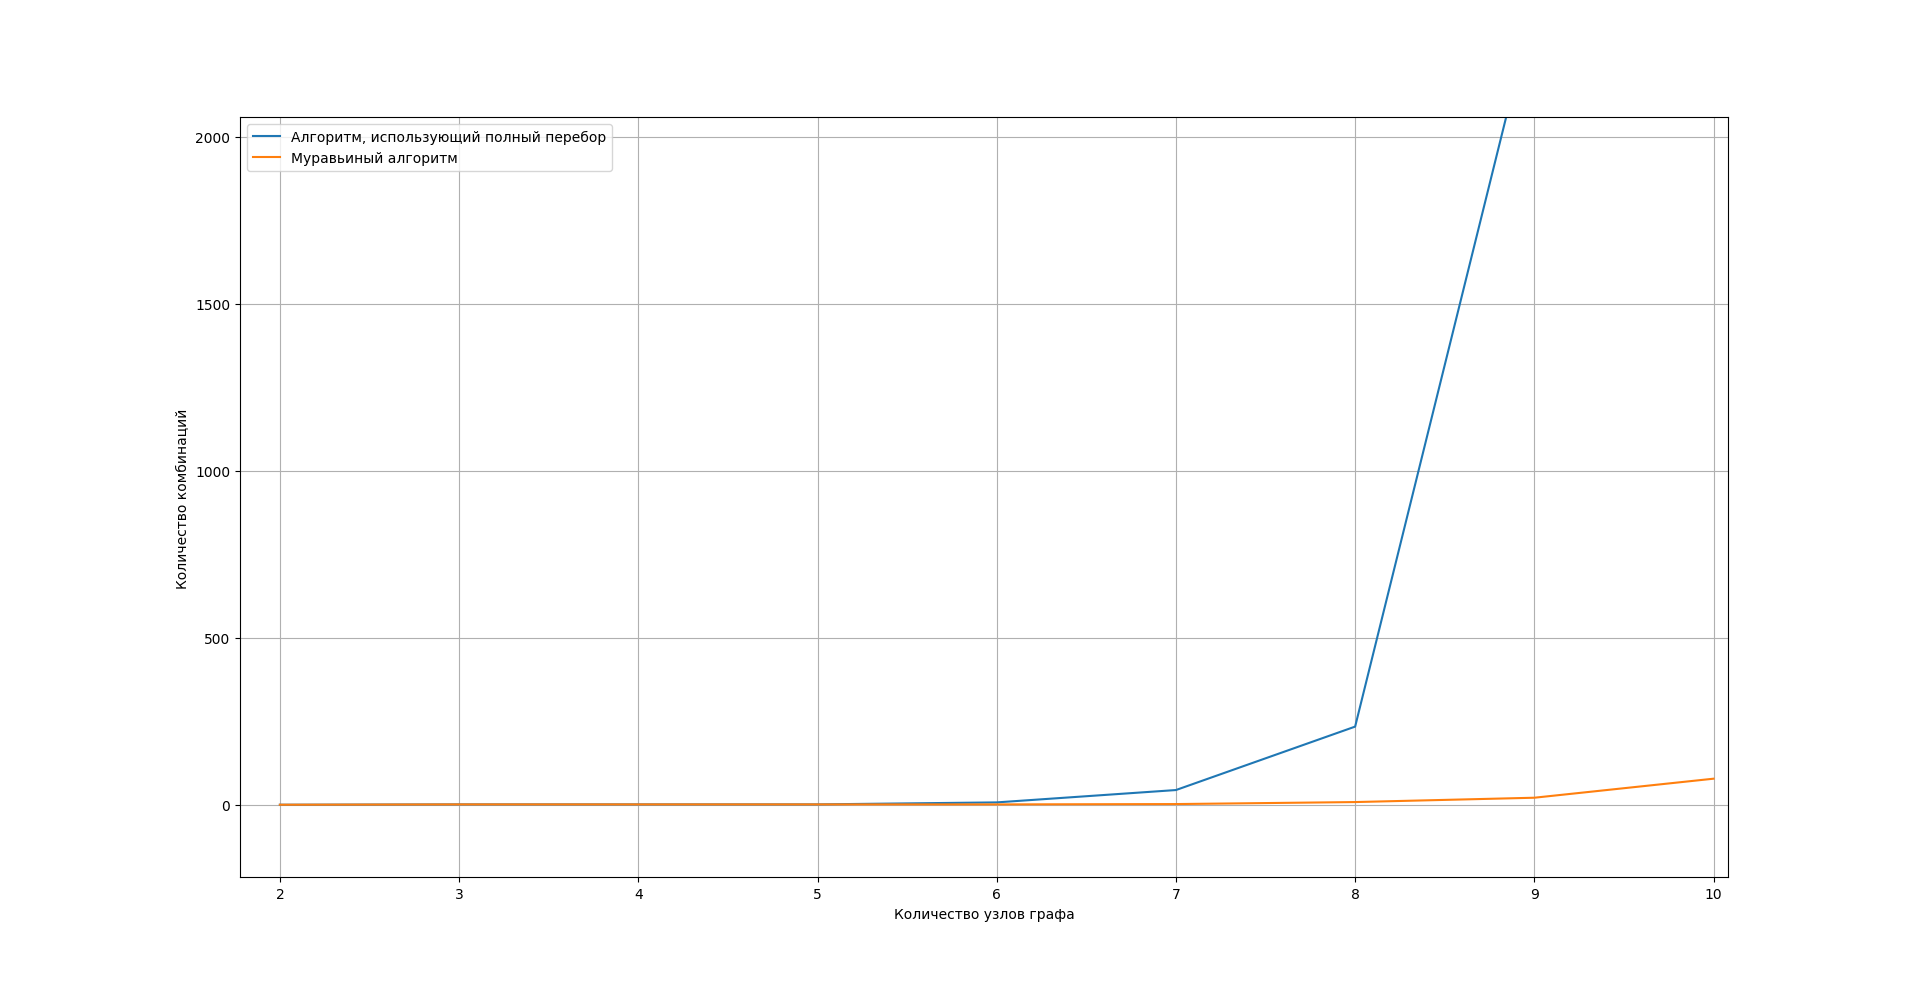
\includegraphics[scale=1]{graphics.png}}
\caption{График зависимости времени работы алгоритмов от длин сторон матриц}
\label{images:graphics}
\end{figure}

\newpage
\subsection{Оценка затрачиваемой памяти}
% Написать оценку затрачиваемой памяти

\newpage
\subsection{Вывод}
% Для начала надо оформить предыдущие разделы



\newpage
\anonsection{ЗАКЛЮЧЕНИЕ}
% Нужно написать и эту каку



\newpage
\anonsection{СПИСОК ИСТОЧНИКОВ}
% ХЗ что ещё брать кроме ХАБРа

\end{document}
